\documentclass[mathserif]{beamer}

\usepackage{thesis}
\usepackage{pdfpages}
\usepackage{array}
\usepackage{booktabs}


\title[Sampling from Probabilistic Submodular Models]
{Sampling from Probabilistic Submodular Models}

\author[Alkis Gotovos]{}


\newcommand{\tab}[2]{%
\makebox[#1\linewidth][l]{#2}%
}

\begin{document}

\setbeamertemplate{background canvas}{}
\vspace{0.5em}
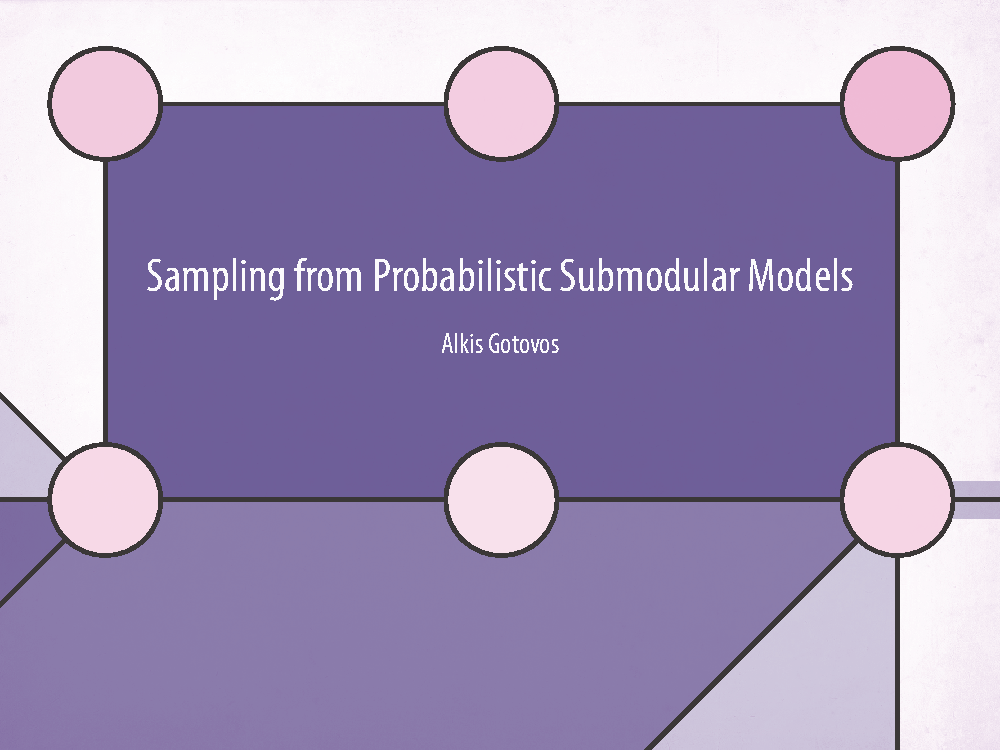
\includepdf[pages={1}]{title/title.pdf}
\setbeamertemplate{background canvas}{
\includegraphics[width=\paperwidth]{figures/bg_no_line.png}}


\begin{frame}{Cancer Pathways}
\centering
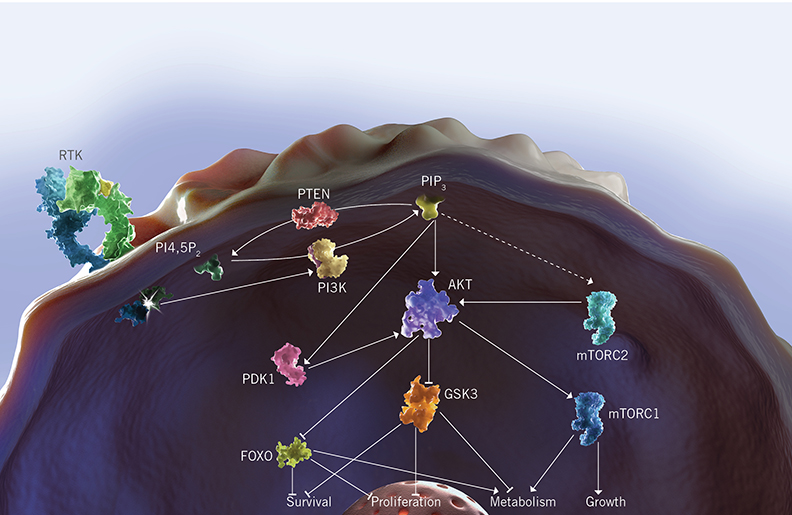
\includegraphics[width=\textwidth]{figures/pathways_pik3k.jpg}\\[-0.3em]
\hfill{}\qsource{biooncology.com}
\end{frame}

\begin{frame}{Goal}
\centering
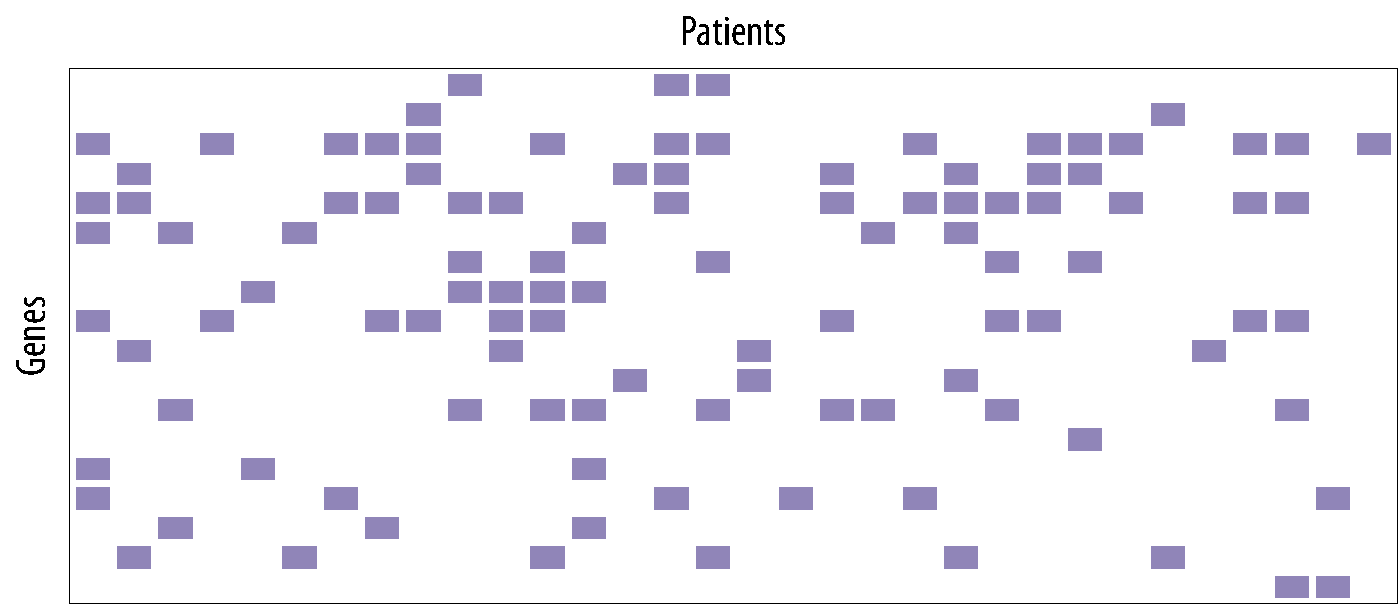
\includegraphics[width=3.7in]{figures/example1.pdf}

\vspace{3em}
\uncover<2>{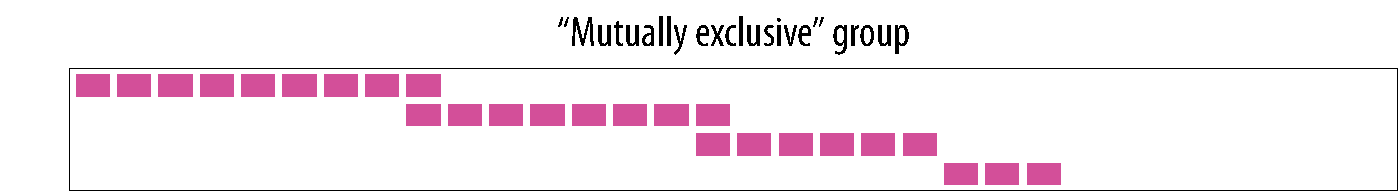
\includegraphics[width=3.7in]{figures/example1_rep_group.pdf}}
\end{frame}

\begin{frame}{Pipeline}
\begin{enumerate}
  \item Preprocess raw data to obtain mutation matrix \uncover<2->{{\color{col2}\& handle missing data}}
  \vspace{1em}
  \item Learn prob. submodular model $\ \ p(S) \propto \exp(F(S; \*u, \*W))$\\[0.5em]
  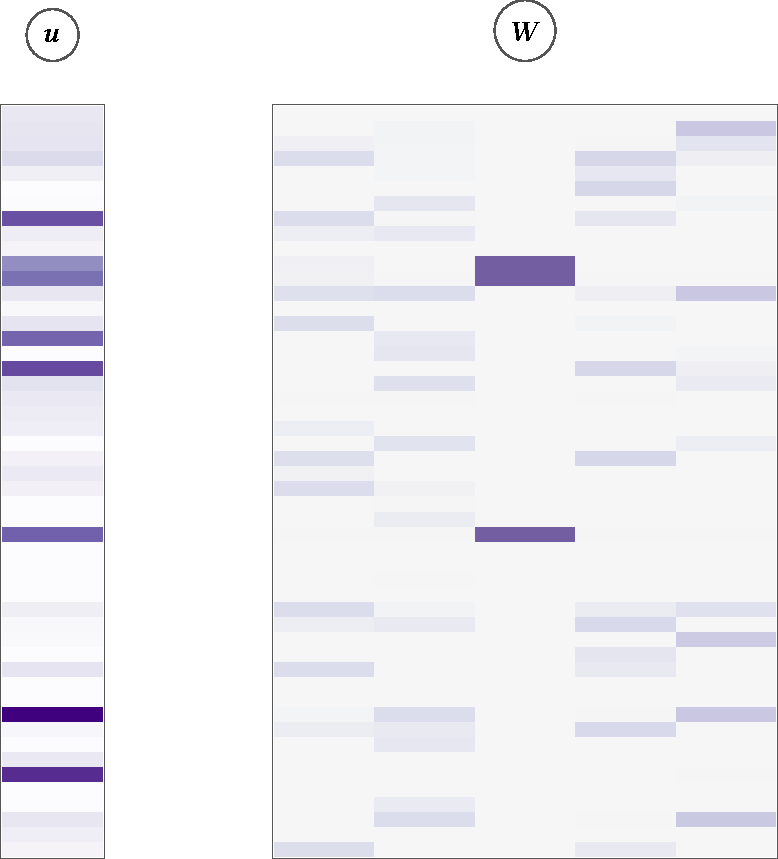
\includegraphics[width=1.3in]{figures/mat_old_reg.pdf}
  \vspace{1em}
  \item Extract candidate mutually exclusive groups
  \vspace{1em}
  \item \alt<1>{Filter groups via statistical tests}{\color{col2}Filter groups via statistical tests}
\end{enumerate}
\end{frame}

\begin{frame}{Missing data}
  \centering
  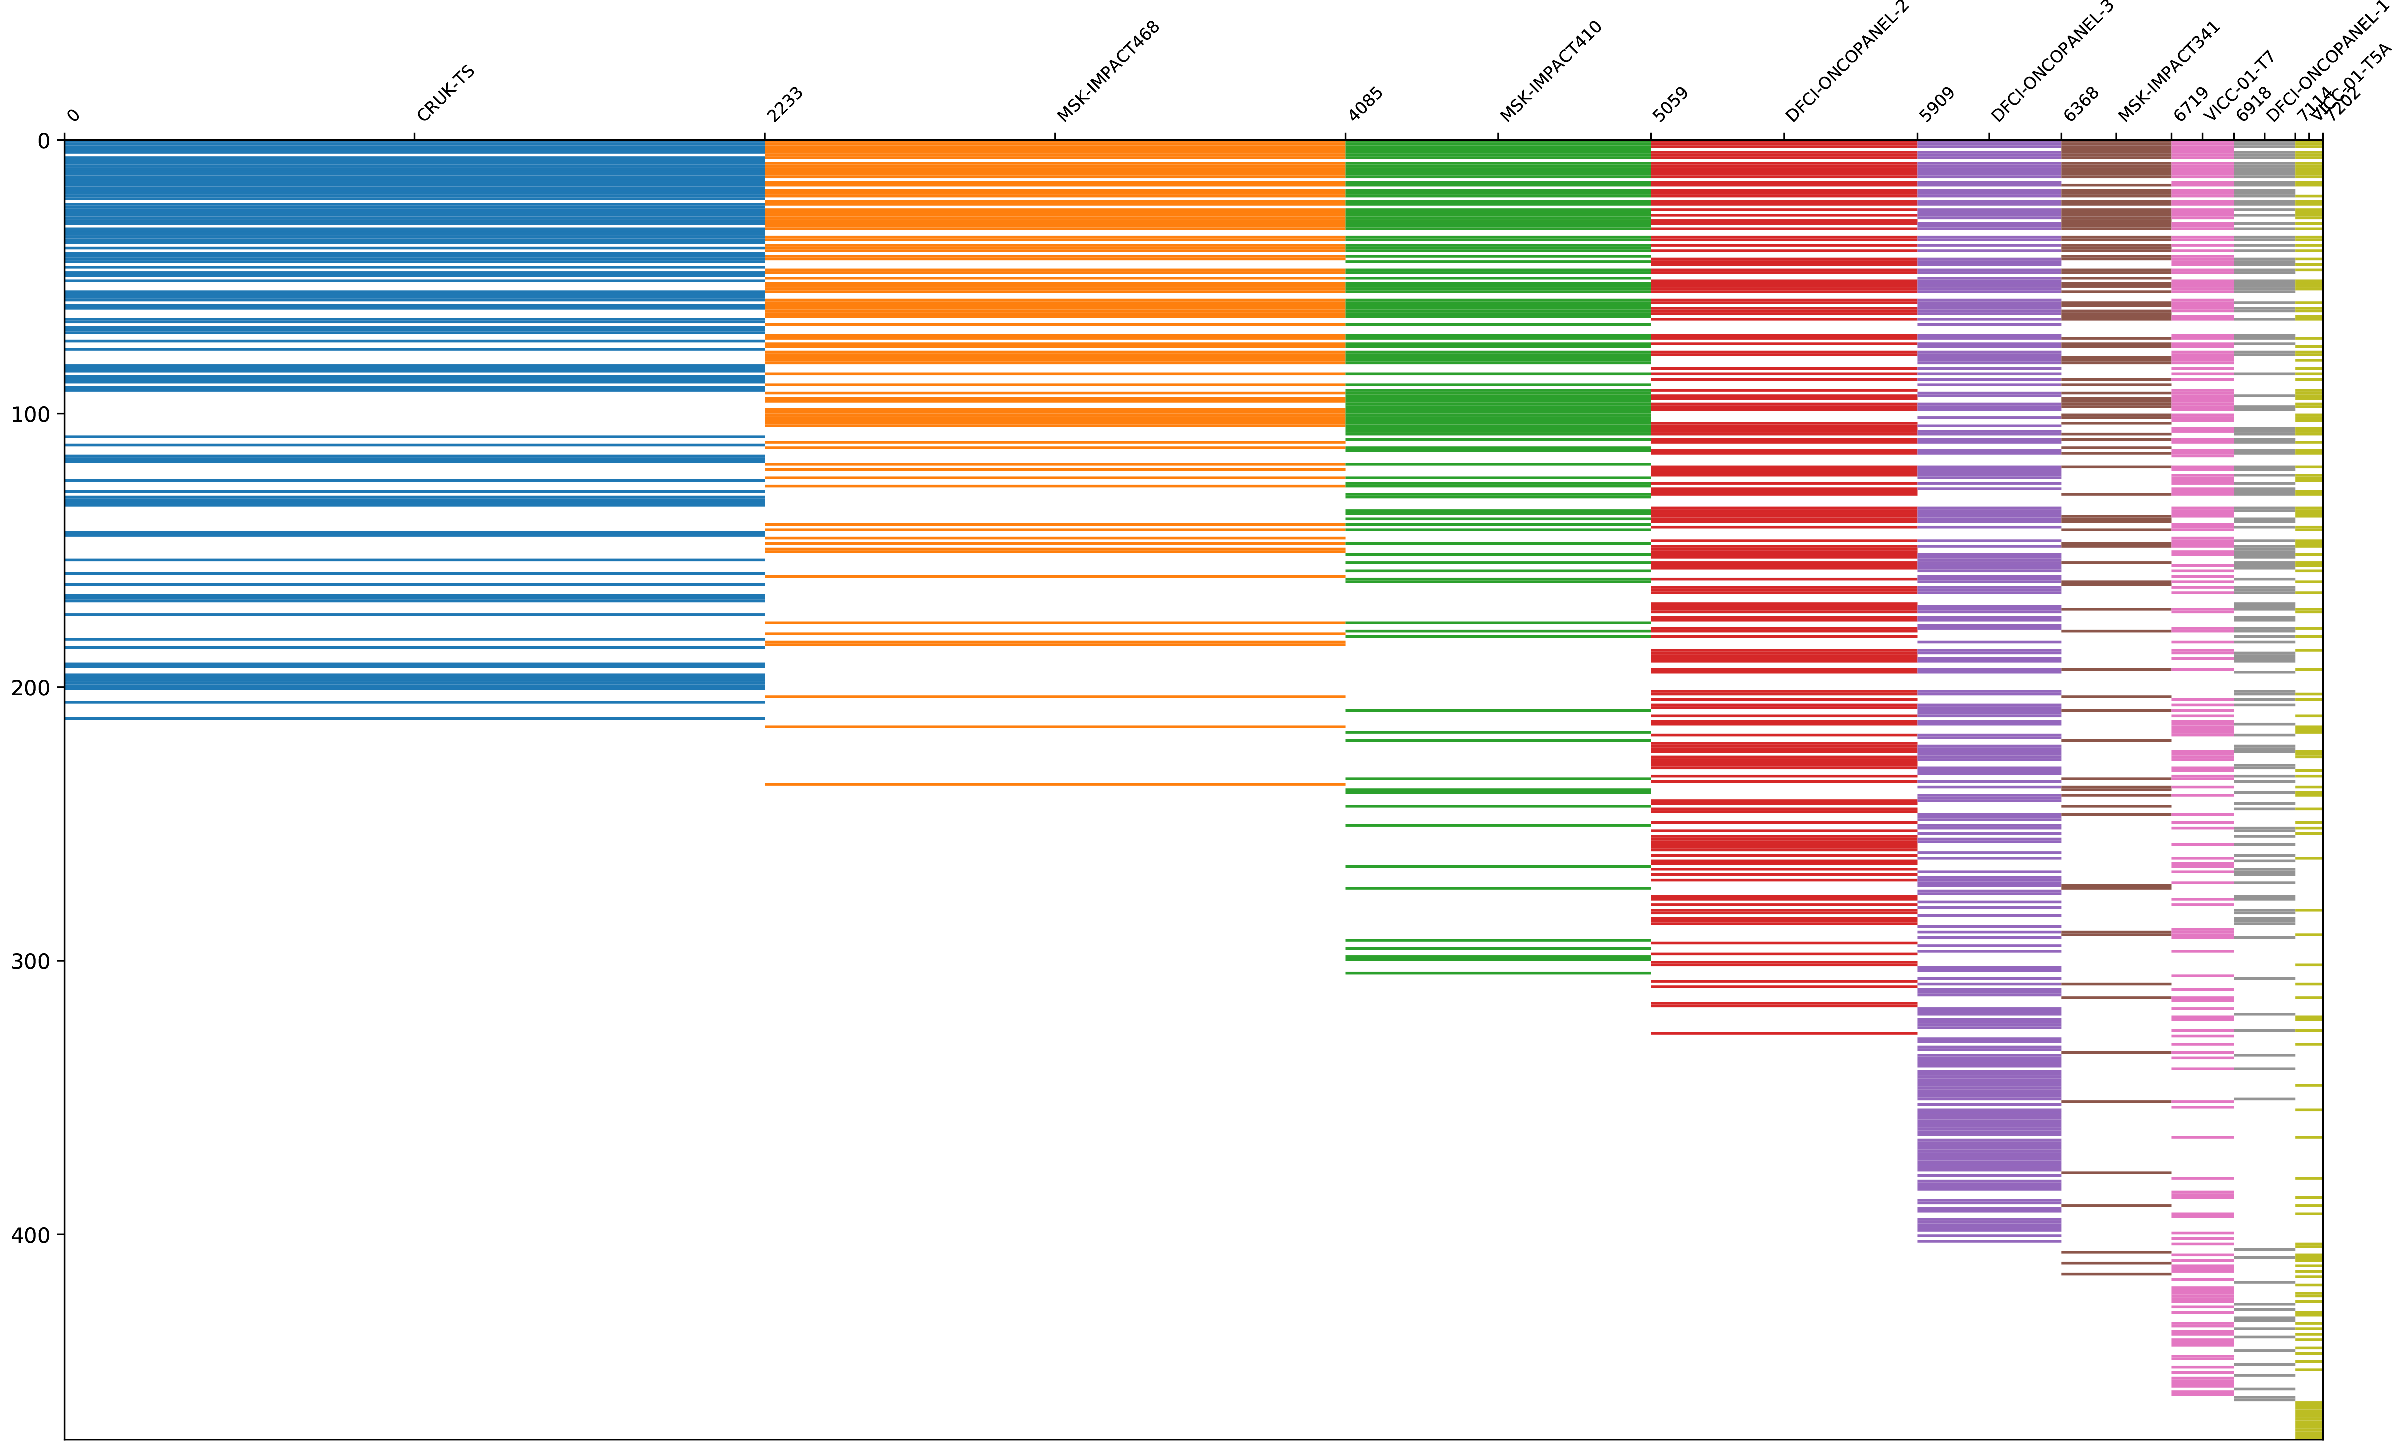
\includegraphics[width=\textwidth]{figures/brca_panels_9.pdf}
\end{frame}

\begin{frame}{Solution I: Panel intersection}
  \centering
  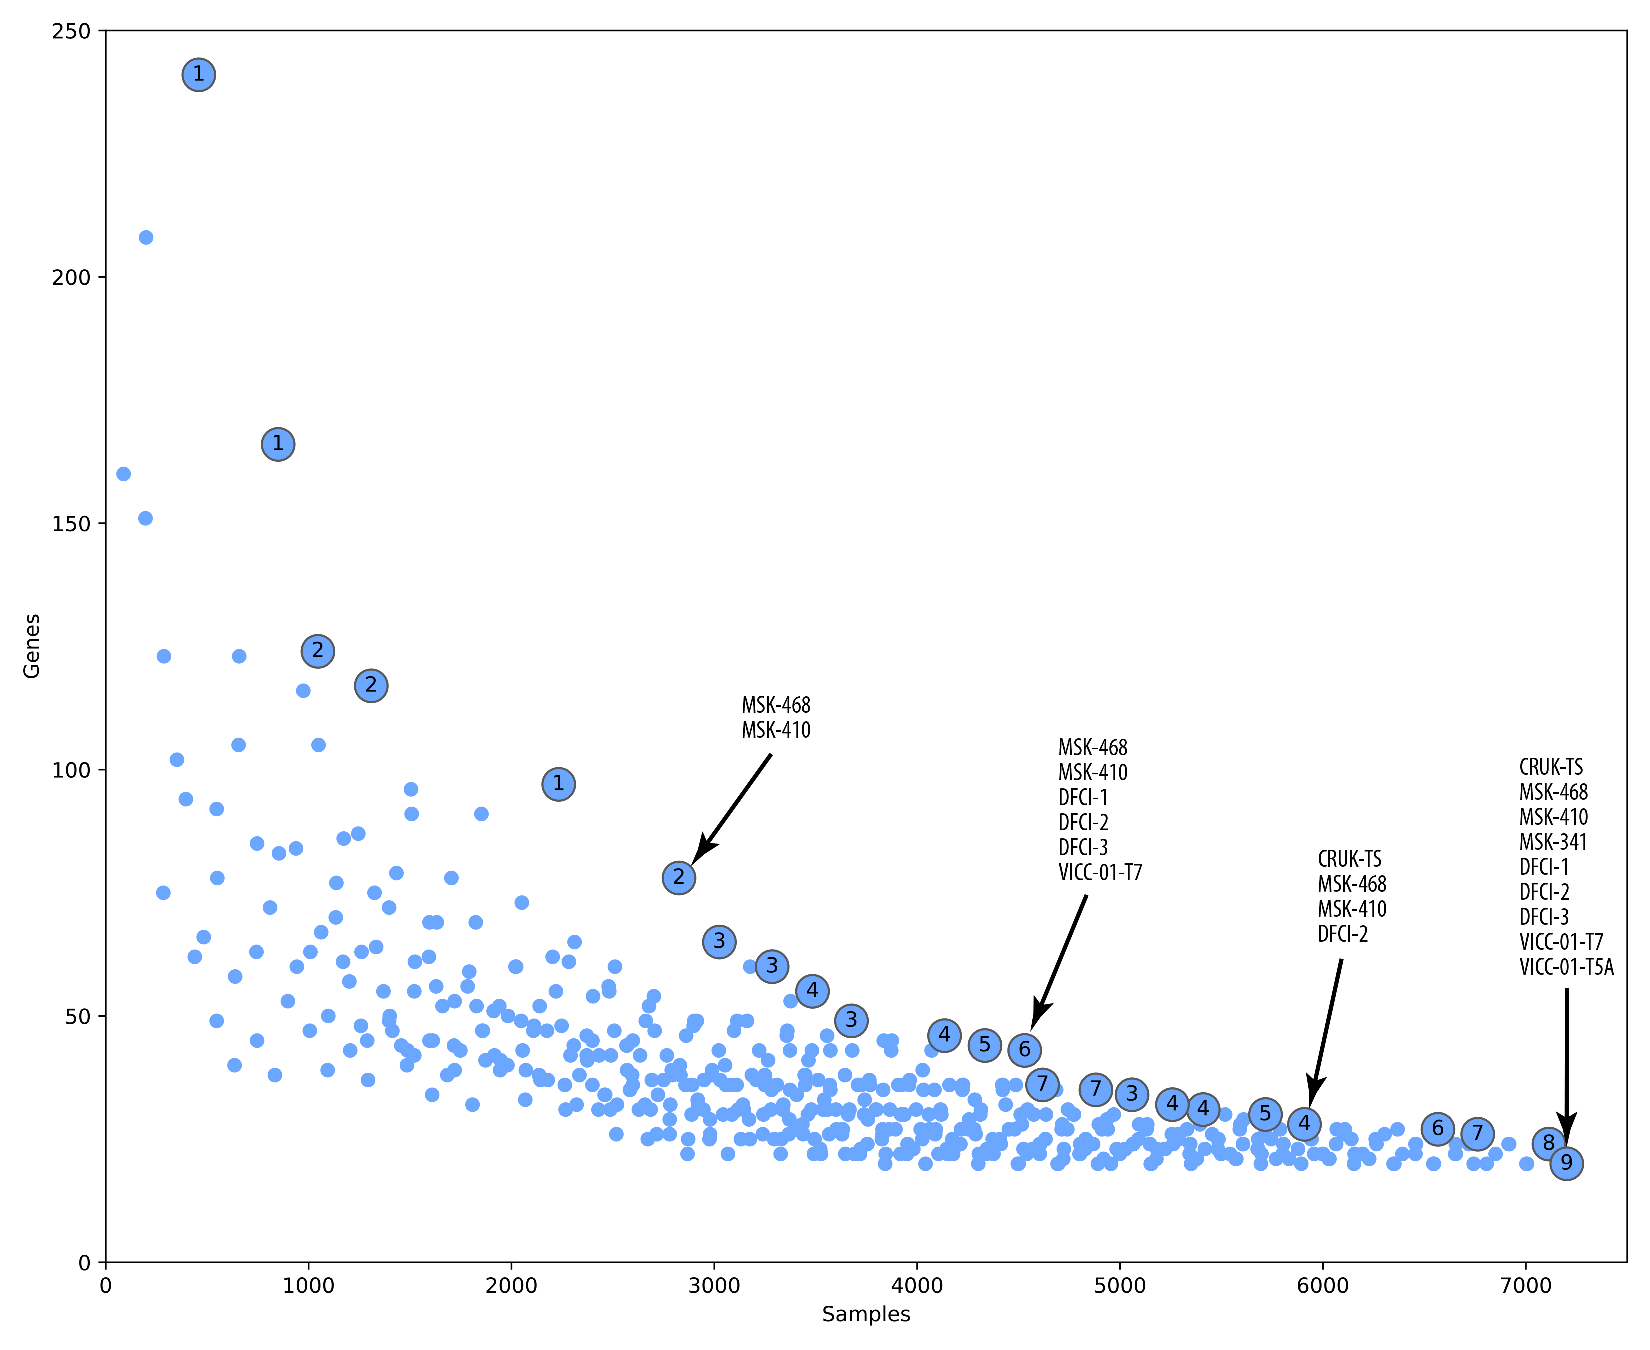
\includegraphics[width=3.8in]{figures/brca_panels_pareto_annotated.pdf}
\end{frame}

\begin{frame}{Solution I: Trivial imputation}
  \centering
  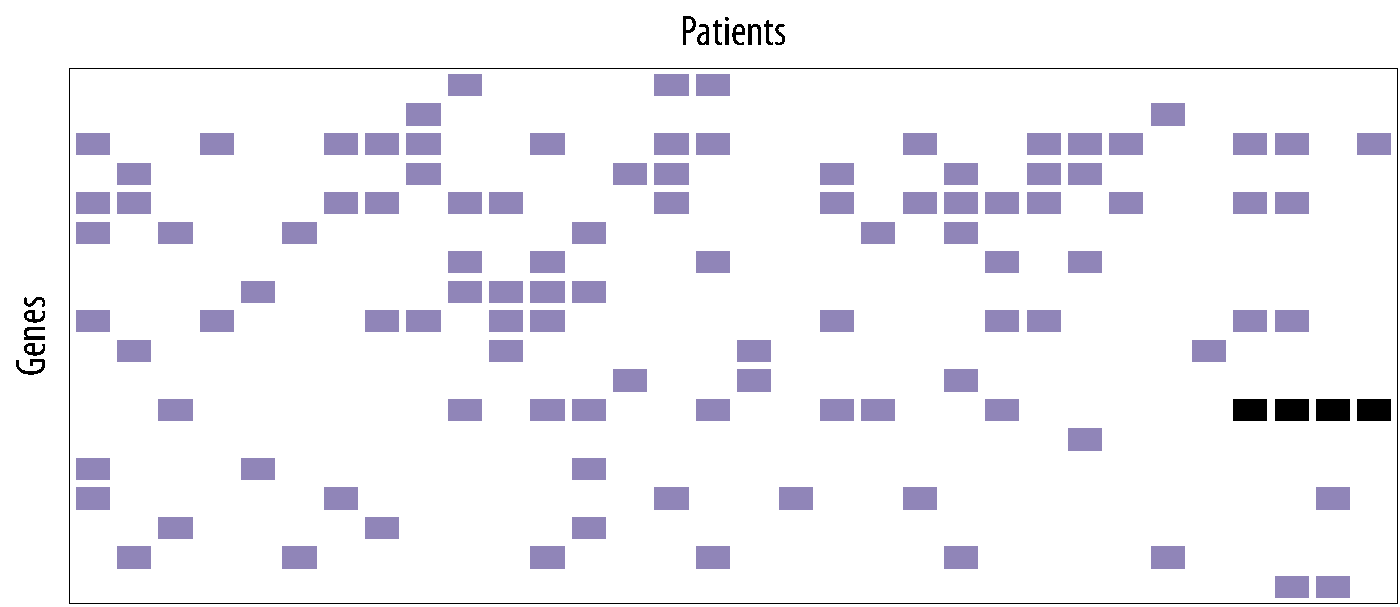
\includegraphics[width=3.7in]{figures/example1_missing.pdf}
\end{frame}

\begin{frame}{Solution II: Trivial imputation}
  \centering
  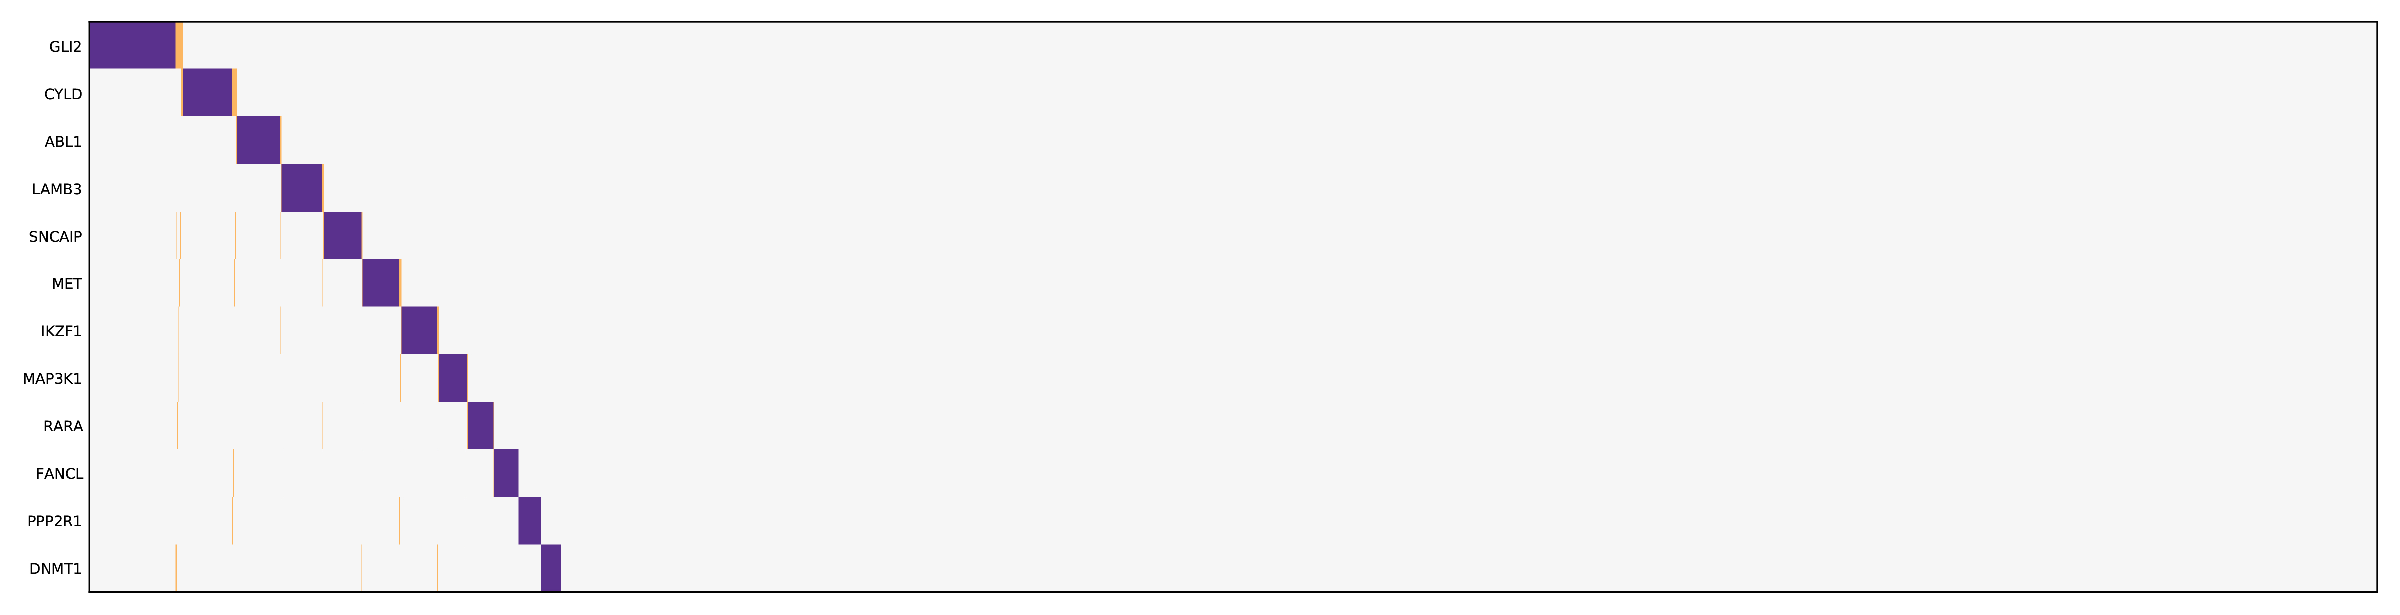
\includegraphics[width=\textwidth]{figures/brca_fill.pdf}
  \vspace{1em}
  \begin{itemize}
	\item May be able to filter it out (more on this later), but\ldots
	\vspace{0.5em}
	\item \ldots extra noise makes filtering more conservative,
	\item \ldots spurious groups occupy space in the representation.
\end{itemize}
\end{frame}

\begin{frame}{Solution III: Trivial multiple imputation}
  \centering
  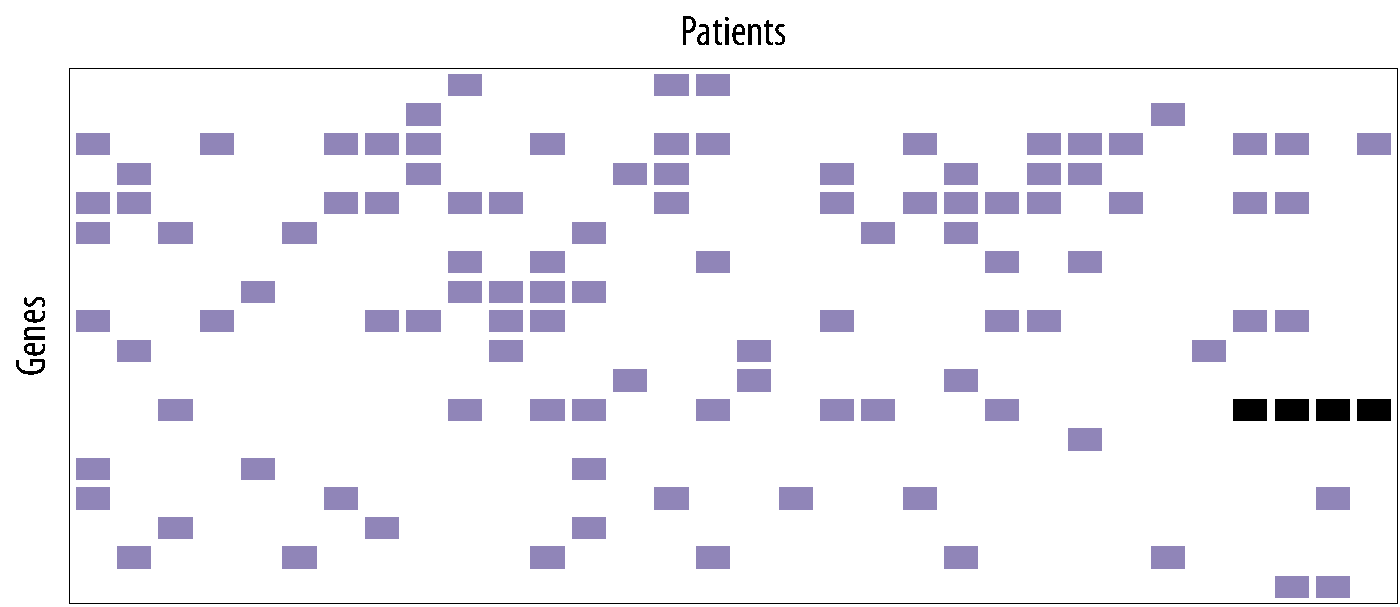
\includegraphics[width=3.7in]{figures/example1_missing.pdf}
  
  \vspace{2em}
  \uncover<2->{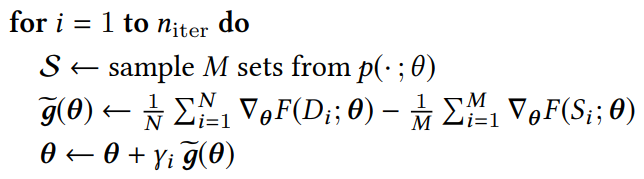
\includegraphics[width=3in]{figures/maxlik.png}}
\end{frame}

\begin{frame}{Solution III: Trivial multiple imputation}
  \centering
  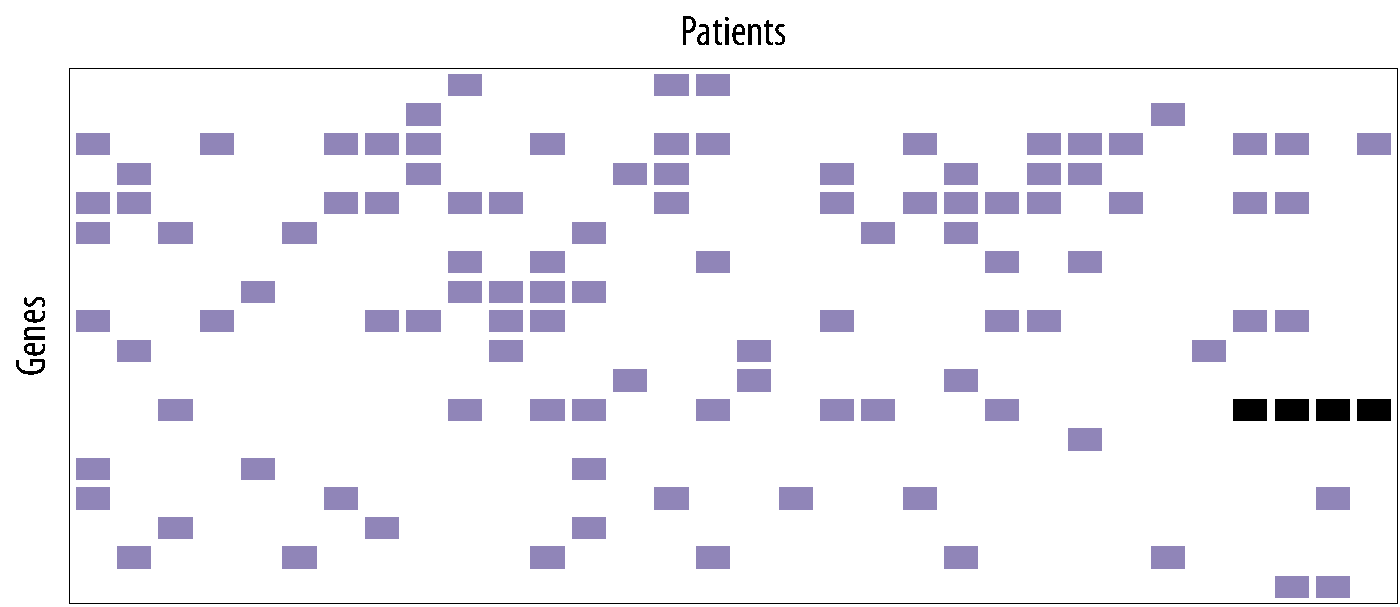
\includegraphics[width=3.7in]{figures/example1_missing.pdf}

  \vspace{2em}
  \uncover<2->{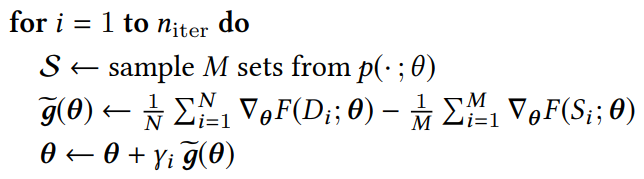
\includegraphics[width=3in]{figures/maxlik.png}}
\end{frame}

\begin{frame}{Solution III: Trivial multiple imputation}
  \centering
  Original data
  \alt<2->{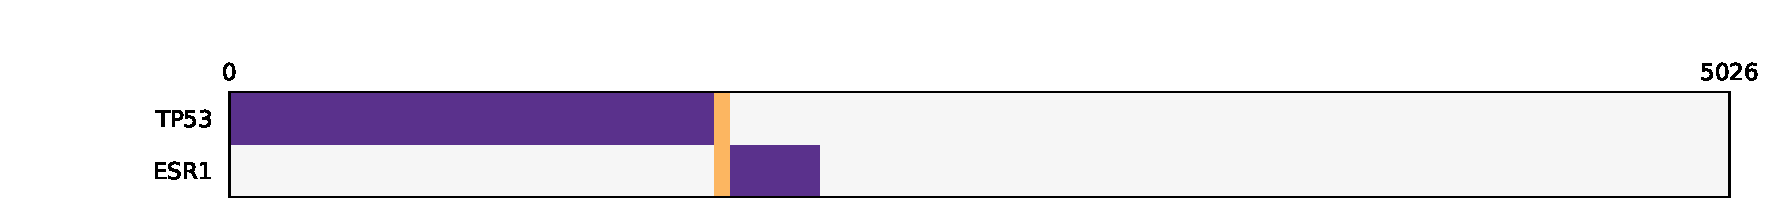
\includegraphics[width=\textwidth,trim={2cm 0 0 1cm},clip]{figures/group_orig_stretched.pdf}}{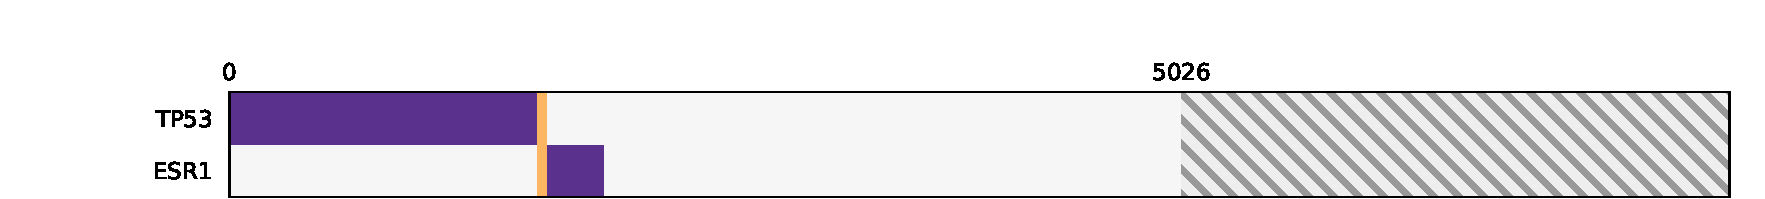
\includegraphics[width=\textwidth,trim={2cm 0 0 1cm},clip]{figures/group_orig.pdf}}
  
  \vspace{3em}
  Imputed data
  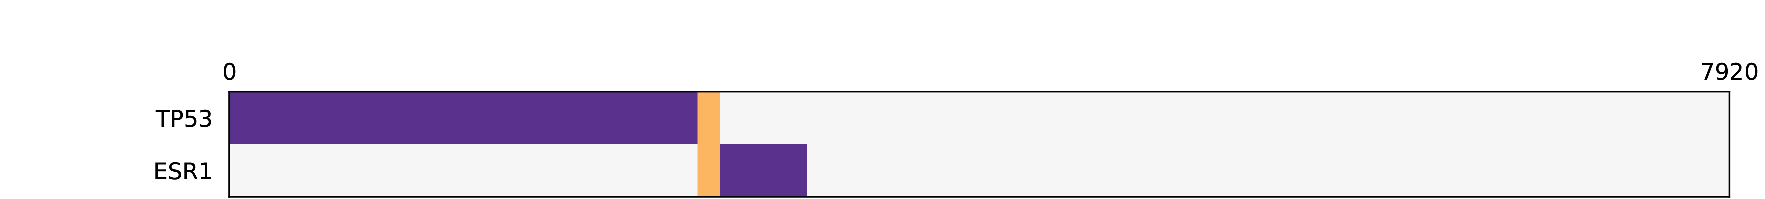
\includegraphics[width=\textwidth,trim={2cm 0 0 1cm},clip]{figures/group_filled.pdf}
\end{frame}

\begin{frame}{Solution IV: Sophisticated multiple imputation}
  \begin{itemize}
    \item Fully-conditional specification: $\ \ P(G_i \mid G_1, \ldots, G_{i-1}, G_{i+1}, G_n, \theta_i)$
    \vspace{1em}
    \item Start with some initial imputation $\hat{G}_i$
    \vspace{1em}
    \item for $t = 1,\ldots,N_{\textrm{iter}}$\\[0.2em]
          \hspace{0.9em}for $i = 1,\ldots, n$
    \vspace{0.5em}
    \begin{itemize}
    	\item Draw $\theta_i \sim P(\cdot \mid G_i, \hat{G}_{-i})$
    	\vspace{0.5em}
    	\item Draw $\hat{G}_i \sim P(\cdot \mid \hat{G}_{-i}, \theta_i)$
    \end{itemize}
  \end{itemize}
  \vspace{2em}
  
  \uncover<2->{%
  \begin{itemize}
  	\item Looks exactly like Gibbs sampling, but implied joint dist. may not exist
  	\vspace{0.5em}
  	\item Surprising lack of ML libraries (e.g., MICE in R)
  	\vspace{0.5em}
  	\item Slow!
  \end{itemize}
  }
  
\end{frame}

\begin{frame}{Solution IV: Sophisticated multiple imputation}
  \centering
  Original data
  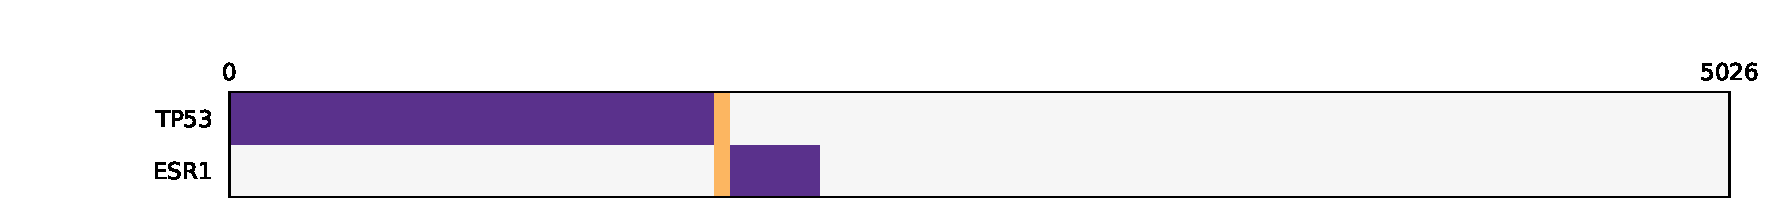
\includegraphics[width=\textwidth,trim={2cm 0 0 1cm},clip]{figures/group_orig_stretched.pdf}

  \vspace{2em}
  Trivially-imputed data
  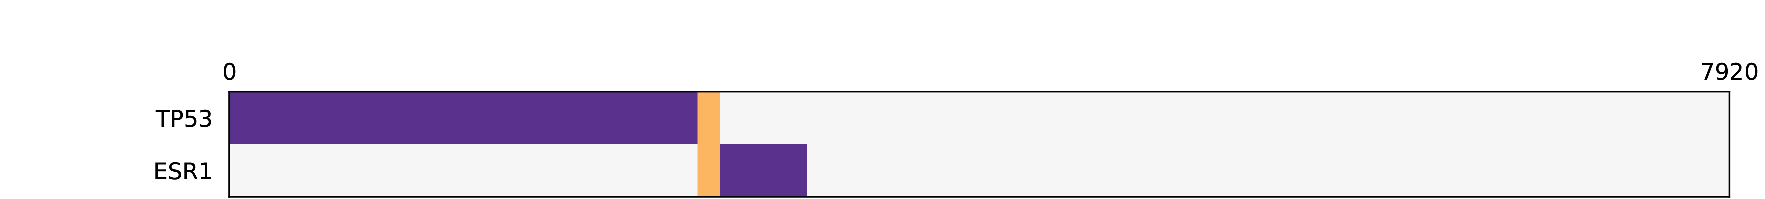
\includegraphics[width=\textwidth,trim={2cm 0 0 1cm},clip]{figures/group_filled.pdf}
  
  \vspace{2em}
  MICE-imputed data
  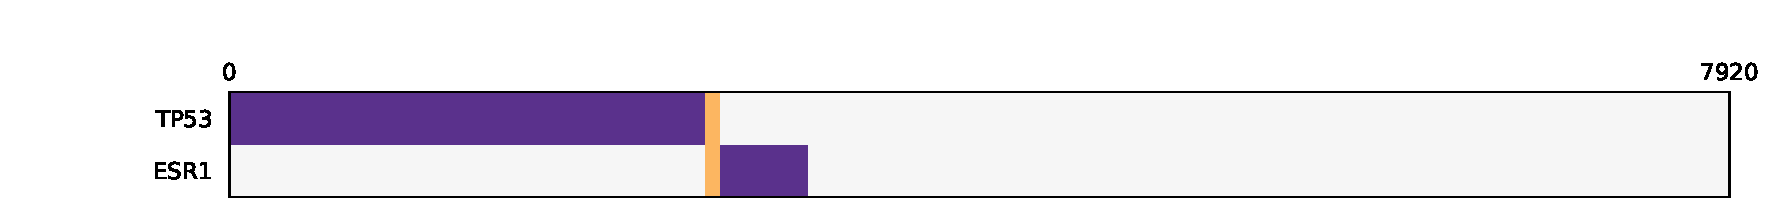
\includegraphics[width=\textwidth,trim={2cm 0 0 1cm},clip]{figures/group_mice.pdf}
\end{frame}

\begin{frame}{Solution V: Marginal learning}
Log-likelihood $\ \ \ell(\theta) = \displaystyle\sum_{i=1}^{N} \log p(D_i; \theta)$
  
\begin{align*}
  \ell(\theta) &= \sum_{i=1}^{N_1} \log p\left(\left(g_1^{(i)}, g_2^{(i)}, \*?\right); \*\theta\right) + \sum_{i=1}^{N_2} \log p\left(\left(g_1^{(i)}, \*?, g_3^{(i)}\right); \*\theta\right)\\
  \ell_{\textrm{marg}}(\theta) &= \sum_{i=1}^{N_1} \log p_{12}\left(\left(g_1^{(i)}, g_2^{(i)}\right); \*\theta\right) + \sum_{i=1}^{N_2} \log p_{13}\left(\left(g_1^{(i)}, g_3^{(i)}\right); \*\theta\right)
\end{align*}

\vspace{1em}
\uncover<4->{%
\centering
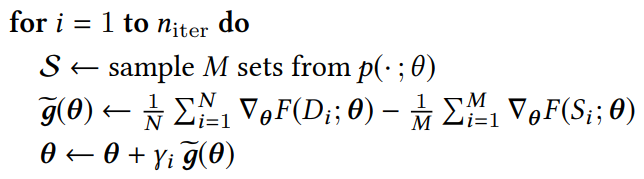
\includegraphics[width=3in]{figures/maxlik.png}%
}
\end{frame}

\begin{frame}{Summary}
\begin{enumerate}[(I)]
  \item {\color{colneg}Panel intersection}
  \vspace{0.7em}
  \item {\color{colneg}Trivial imputation}
  \vspace{0.7em}
  \item {\color{colneg}Trivial multiple imputation}
  \vspace{0.7em}
  \item {\color{colpos}Sophisticated multiple imputation}
  \vspace{0.7em}
  \item {\color{colpos}Marginal learning}
\end{enumerate}
\end{frame}

\end{document}
